%!TEX TS-program = xelatex
%!TEX encoding = UTF-8 Unicode
%& -bibtex
%
% $Id: cjcmsample.tex,v 1.5 2007/06/05 02:59:29 zlb Exp $

% 文档类选项:
%   draft   - 草稿模式 (缺省)
%   final   - 终稿模式
%   jssx    - 《计算数学》(缺省)
%   szjs    - 《数值计算与计算机应用》
\documentclass[szjs]{cjcmltx}

%
%       M A C R O S
%
%       Operators
\usepackage{amsmath,amssymb,amsfonts,algorithm, algorithmicx, algpseudocode}
\usepackage{graphicx,color,tikz}

\let\mathbf\boldsymbol
\newcommand\curl{\mathop{\mathbf{\nabla}\times}}
\newcommand\grad{\mathop{\mathbf{\nabla}}}
\renewcommand\div{\mathop{\mathbf{\nabla}\cdot}}
\newcommand{\E}{\mathbf{E}}
\newcommand{\J}{\mathbf{J}}

\def\vec#1{\mathbf{#1}}
\def\R{\mathbb{R}}
\def\C{{\mathscr C}}

\newcommand{\bcurl}{\mathbf{curl}}
\renewcommand{\i}{{\rm\mathbf i}}
\newcommand{\lj}{[{\hskip -2pt} [}
\newcommand{\rj}{]{\hskip -2pt} ]}
\newcommand{\xa}[2]{\|\, #1 \,\|_{L^2({#2})}}

\def\fig{figure}
\floatname{algorithm}{算法}
\renewcommand{\algorithmicrequire}{\bf 输入: }
\renewcommand{\algorithmicensure}{\bf 输出: }
\begin{document}

\def\Jvol{}
\def\Jno{}
\def\Jyear{2020}
\def\Jmonth{11}
\def\Jreceived{~	}
\def\Jrevised{}

\def\Term{中国科学院大学2020\ -\ 2021学年秋季学期}
\def\Major{计算数学}
\def\Aid{201928000206026}

\setcounter{page}{1}

%------------------------ 中文标题、摘要 --------------------------

\markright{并行计算导论}

\title{Strassen算法的并行化实现}

\author{廖钰蕾\affiliation{LSEC, 中国科学院, 数学与系统科学研究院,
                         计算数学与科学工程计算研究所, 北京~100190}
    }

\maketitle

\begin{abstract}
矩阵乘法是科学计算中必不可少的部分, 经典的三层循环算法时间复杂度为$O(N^3)$. 事实上, 还有一些时间复杂度低于$O(N^3)$的工作, 例如Strassen算法, 以及Winograd变体等, 渐进复杂度为$O(N^{2.81})$. 本文对Strassen算法进行了并行化实现与测试. 在CPU环境下的openMP实现中, 通过测试选取合适的参数后, 在大规模矩阵下的计算速度相比经典的$O(N^3)$时间复杂度矩阵乘法有明显提高, 在大规模矩阵下的效率能保持在60\%以上, 扩展性较好. 在GPU环境下的CUDA实现中, 经典的三层循环方法已经能达到很好的计算效率, 并且随着矩阵规模增大, GPU的浮点运算性能显著提高.
\end{abstract}

\begin{keywords}
Strassen算法\ \ \ \ 并行计算\ \ \ \ openMP\ \ \ \ CUDA
\end{keywords}

\section{问题描述}
矩阵乘法是科学计算中必不可少的部分. 常见的加速方法是基于经典的三层循环算法, 通过行划分, 列划分, 快划分等方式并行实现, 其串行算法时间复杂度为$O(N^3)$, 其中$N$是矩阵行列规模. 

事实上, 还有一些时间复杂度低于$O(N^3)$的工作, 例如Strassen算法~\cite{Strassen:1969}, 以及Winograd变体~\cite{Winograd:1971}等, 这两个算法的渐进复杂度为$O(N^{2.81})$. 我们关注的即是Strassen算法的在CPU上的openMP实现, 以及在GPU上的CUDA实现~\cite{Li:2011}.

 Strassen算法涉及递归调用, 递归层数过深或过浅都会影响算法效率. 我们通过测试选取不同并行平台上的合适参数, 并测试并行算法的加速比, 并行效率, 强可扩展性, 弱可扩展性, 浮点运算性能等并行性能.

\section{数学模型}
计算矩阵乘法$C=AB$, 其中$A, B, C\in\R^{N\times N}$. 为了简单起见, 我们假设$N=2^k$, 其中$k$是非负整数. 其它情形可以通过填充0实现.


Strassen算法的基本思想是按图~\ref{fig:block}的方式划分矩阵, 再按下述公式计算~\cite{Strassen:1969}:
\begin{align*}
& M_1=(A_{11}+A_{22})(B_{11}+B_{22}),\\
& M_2=(A_{21}+A_{22})B_{11}, && C_{11}=M_1+M_4-M_5+M_7,\\
& M_3=A_{11}(B_{12}-B_{22}), && C_{12}=M_3+M_5,\\
& M_4=A_{22}(B_{21}-B_{11}), && C_{21}=M_2+M_4,\\
& M_5=(A_{11}+A_{12})B_{22}, && C_{22}=M_1-M_2+M_3+M_6.\\
& M_6=(A_{21}-A_{11})(B_{11}+B_{12}),\\
& M_7=(A_{12}-A_{22})(B_{21}+B_{22}),\\
\end{align*}
等式中的矩阵乘均为递归调用. 注意到递归调用该方法时, 会产生很多临时的矩阵$M_i$, 可以通过在每一层递归调用中使用2个临时矩阵解决这一问题~\cite{Douglas:1994}.

\begin{figure}[htbp]\centering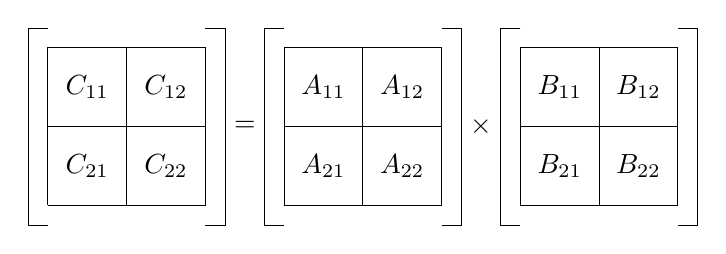
\begin{tikzpicture}
\draw(0,0)--(2,0)--(2,2)--(0,2)--(0,0);
\draw(0,1)--(2,1);
\draw(1,0)--(1,2);
\node at(0.5,1.5){$C_{11}$};
\node at(1.5,1.5){$C_{12}$};
\node at(0.5,0.5){$C_{21}$};
\node at(1.5,0.5){$C_{22}$};
\draw(3,0)--(5,0)--(5,2)--(3,2)--(3,0);
\draw(3,1)--(5,1);
\draw(4,0)--(4,2);
\node at(3.5,1.5){$A_{11}$};
\node at(4.5,1.5){$A_{12}$};
\node at(3.5,0.5){$A_{21}$};
\node at(4.5,0.5){$A_{22}$};
\draw(6,0)--(8,0)--(8,2)--(6,2)--(6,0);
\draw(6,1)--(8,1);
\draw(7,0)--(7,2);
\node at(6.5,1.5){$B_{11}$};
\node at(7.5,1.5){$B_{12}$};
\node at(6.5,0.5){$B_{21}$};
\node at(7.5,0.5){$B_{22}$};
\draw(0,2.25)--(-0.25,2.25)--(-0.25,-0.25)--(0,-0.25);
\draw(2,2.25)--(2.25,2.25)--(2.25,-0.25)--(2,-0.25);
\draw(3,2.25)--(2.75,2.25)--(2.75,-0.25)--(3,-0.25);
\draw(5,2.25)--(5.25,2.25)--(5.25,-0.25)--(5,-0.25);
\draw(6,2.25)--(5.75,2.25)--(5.75,-0.25)--(6,-0.25);
\draw(8,2.25)--(8.25,2.25)--(8.25,-0.25)--(8,-0.25);
\node at(2.5,1){$=$};
\node at(5.5,1){$\times$};
\end{tikzpicture}
\caption{$A,B,C$的矩阵划分}\label{fig:block}
\end{figure}

\section{数值方法}
\subsection{串行算法}
Strassen算法的渐进时间复杂度为$O(N^{2.81})$, 然而在实际计算中, 临时矩阵的生成与释放, 以及递归过程会耗费大量的时间. 因此我们实际考虑的是带参数的Strassen算法~\cite{Li:2011}. 具体算法由零层实现, 一层实现, 多层实现三部分组成.

\subsubsection{零层实现}
零层实现采用时间复杂度为$O(N^3)$的经典三层嵌套矩阵乘法. 定义核函数mul计算$A\times B$, 见表~\ref{tab:zero}.

\begin{table}[htbp]\centering\caption{零层实现}\label{tab:zero}
\begin{tabular}{|l|l|l|}
\hline
步骤 & 操作& 核函数\\
\hline
1 & $C=A\times B$ & mul($A, B, C$)\\
\hline
\end{tabular}
\end{table}

\subsubsection{一层实现}
一层实现采用非递归调用的Strassen算法~\cite{Strassen:1969}, 其复杂度仍为$O(N^3)$, 但复杂度隐藏的常数项不同. 具体实现见表~\ref{tab:one}.
\begin{table}[htbp]\centering\caption{一层实现}\label{tab:one}
\begin{tabular}{|l|l|l|}
\hline
步骤 & 操作& 核函数\\
\hline
1 & $[A_{11},A_{12};A_{21},A_{22}]=A$ & split($A_{11},A_{12},A_{21},A_{22},A$)\\
\hline
2 & $[B_{11},B_{12};B_{21},B_{22}]=B$ & split($B_{11},B_{12},B_{21},B_{22},B$)\\
\hline
3 & $T_1=A_{11}-A_{21}$ & sub($A_{11},A_{21},T_1$)\\
\hline
4 & $T_2=B_{22}-B_{12}$ & sub($B_{22},B_{12},T_2$)\\
\hline
5 & $C_{21}=T_1\times T_2$ & mul($T_1,T_2,C_{21}$)\\
\hline
6 & $T_1=A_{21}+A_{22}$ & add($A_{21},A_{22},T_1$)\\
\hline
7 & $T_2=B_{12}-B_{11}$ & sub($B_{12},B_{11},T_2$)\\
\hline
8 & $C_{22}=T_1\times T_2$ & mul($T_1,T_2,C_{22}$)\\
\hline
9 & $T_1=T_1-A_{11}$ & sub($T_1,A_{11},T_1$)\\
\hline
10 & $T_2=B_{22}-T_2$ & sub($B_{22},T_2,C_{22}$)\\
\hline
11 & $C_{11}=T_1\times T_2$ & mul($T_1,T_2,C_{11}$)\\
\hline
12 & $T_1=A_{12}-T_1$ & sub($A_{12},T_1,T_1$)\\
\hline
13 & $C_{12}=T_1\times B_{22}$ &\\
14 & $C_{12}=C_{22}+C_{12}$ & mul\_add($T_1,B_{22},C_{22},C_{12}$)\\
\hline
15 & $T_1=A_{11}\times B_{11}$ &\\
16 & $C_{11}=C_{11}+T_1$ &\\
17 & $C_{12}=C_{11}+C_{12}$ &\\
18 & $C_{11}=C_{11}+C_{21}$ & mul\_inc\_inc\_inc($A_{11},B_{11},T_1,C_{21},C_{11},C_{12}$)\\
\hline
19 & $T_2=T_2-B_{21}$ & sub($T_2,B_{21},T_2$)\\
\hline
20 & $C_{21}=A_{22}\times T_2$ &\\
21 & $C_{21}=C_{11}-C_{21}$ &\\
22 & $C_{22}=C_{11}+C_{22}$ & mul\_sub\_inc($A_{22},T_2,C_{11},C_{21},C_{22}$)\\
\hline
23 & $C_{11}=A_{12}\times B_{21}$ &\\
24 & $C_{11}=T_1+C_{11}$ & mul\_add($A_{12},B_{21},T_1,C_{11}$)\\
\hline 25 & $C=[C_{11},C_{12};C_{21},C_{22}]$ & merge($C_{11},C_{12},C_{21},C_{22},C$)\\
\hline
\end{tabular}
\end{table}

\subsubsection{多层实现}
多层实现采用递归调用的Strassen算法~\cite{Li:2011}, 具体过程见算法~\ref{alg:strassen}, 算法中调用了零层实现以及一层实现中定义的核函数. 算法中的参数值$\tau_1,\tau_2$待确定.
\begin{algorithm}[htbp]\caption{Strassen算法}\label{alg:strassen}\begin{algorithmic}
\Require 矩阵$A,B,C\in\R^{N\times N}$, 矩阵规模$N$.
\Ensure 矩阵$C\in\R^{N\times N}$.
\Function{Strassen}{$A,B,C,N$}
\If{$N\leq\tau_1$}
\State 调用零层实现
\ElsIf{$N\leq \tau_2$}
\State 调用一层实现
\Else
\State split($A_{11},A_{12},A_{21},A_{22},A$); split($B_{11},B_{12},B_{21},B_{22},B$);
\State sub($A_{11},A_{21},T_1$); sub($B_{22},B_{12},T_2$); Strassen($T_1,T_2,C_{21},N/2$); 
\State add($A_{21},A_{22},T_1$); sub($B_{12},B_{11},T_2$); Strassen($T_1,T_2,C_{22},N/2$);
\State sub($T_1,A_{11},T_1$); sub($B_{22},T_2,C_{22}$); Strassen($T_1,T_2,C_{11},N/2$)
\State sub($A_{12},T_1,T_1$);
\State Strassen($T_1,B_{22},C_{12},N/2$); add($C_{22},C_{12},C_{12}$); //mul\_add
\State Strassen($A_{11},B_{11},T_1,N/2$); add($C_{11},T_1,C_{11}$);
\State add($C_{11},C_{12},C_{12}$); add($C_{11},C_{21},C_{11}$); //mul\_inc\_inc\_inc
\State sub($T_2,B_{21},T_2$);
\State Strassen($A_{22},T_2,C_{21},N/2$); sub($C_{11},C_{21},C_{21}$);
\State add($C_{11},C_{22},C_{22}$); //mul\_sub\_inc
\State Strassen($A_{12},B_{21},C_{11},N/2$); add($T_1,C_{11},C_{11}$); //mul\_add
\State merge($C_{11},C_{12},C_{21},C_{22},C$);
\EndIf
\State\Return $C$
\EndFunction
\end{algorithmic}\end{algorithm}

\subsection{并行化策略}
并行化策略是将零层实现与一层实现中定义的核函数并行实现. 

为了充分利用缓存提高速度, 在openMP实现中, 对于split, merge, add, sub等操作, 采用行划分分配到各个线程, 对于mul, mul\_add, mul\_sub\_inc, mul\_inc\_inc\_inc等含有矩阵乘法运算的操作, 采用列划分分配到各个线程.

在CUDA实现中, 我们选定每个线程块的大小为$m\times m$, 线程块的个数为$\lceil n/m\rceil\times\lceil n/m\rceil$, 其中$n$为核函数所操作的矩阵规模. 具体到每一个线程只负责计算矩阵中一个元素的值.

\section{数值算例: openMP}
\subsection{实验介绍}
实验平台科学与工程计算国家重点实验室的LSSC-IV四号集群系统, 其超算部分主体包含408台新一代ThinkSystem SD530模块化刀片, 每个刀片包括2颗主频为2.3GHz的Intel Xeon Gold 6140 18核Purley处理器和192GB内存, 总共拥有14688个处理器核, 理论峰值性能为1081TFlops, 实测LINPACK性能703TFlops. 操作系统为Red Hat Enterprise Linux Server 7.3.

我们首先通过实验确定合适的参数值$\tau_1,\tau_2$, 之后在考察并行性能指标有:
\begin{itemize}
\item 加速比: 串行执行时间$T_S$与并行执行时间$T_P$的比值$T_S/T_P$.
\item 效率: 加速比与线程数的比值, 即$E_P=T_S/(P\times T_P)$. 其中$P$为并行程序执行进程数.
\item 强可扩展性: 保持总体计算规模不变, 随着线程个数的增加, 观察加速比与效率的变化.
\item 弱可扩展性:保持单个线程的计算规模不变, 随着线程个数的增加,观察加速比与效率的变化.
\end{itemize}

由于openMP是通过创建线程并行, 我们所有的实验都是在一个节点上进行, 不考虑跨节点通信. 为了减小测试误差, 我们连续进行10次迭代, 再取平均值作为结果. 矩阵$A,B$的数值随机生成.

\subsection{确定参数值}
我们通过测试确定参数值$\tau_1,\tau_2$, 考虑线程数为16, 不同矩阵规模$N$下的运行时间见表~\ref{tab:3}. 

\begin{table}[htbp]\centering\caption{线程数16, 不同矩阵规模的运行时间}\label{tab:3}
\begin{tabular}{|c|c|c|c|c|c|c|c|c|}\hline
$\tau_1,\tau_2\backslash N$ & 32 & 64 & 128 & 256 & 512 & 1024 & 2048 & 4096\\
\hline
$\infty,\infty$ & 5.70e-5 & 1.67e-4 & 3.01e-3 & 8.84e-3 & 8.62e-2 & 9.63e-1 & 10.38 & 196.83\\
\hline
$1,\infty$ &5.46e-4 & 1.78e-3 & 1.07e-3 & 7.83e-3 & 5.59e-2 & 6.24e-1 & 9.16 & 80.15\\
\hline
$64,\infty$ & 5.70e-5 & 1.67e-4 & 1.07e-3 & 7.83e-3 & 5.59e-2 & 6.24e-1 & 9.16 & 80.15\\
\hline
$64,64$ & 5.70e-5 & 1.67e-4 & 1.86e-3 & 1.06e-2 & 7.63e-2 & 5.54e-1 & 3.88 & 28.77\\
\hline
$64,512$ & 5.70e-5 & 1.67e-4 & 1.07e-3 & 7.83e-3 & 5.59e-2 & 4.14e-1 & 2.93 & 21.38\\
\hline
\end{tabular}
\end{table}

首先测试$\tau_1=\tau_2=\infty$和$\tau_1=1,\tau_2=\infty$的运行时间, 前者在不同矩阵规模$N$均采用零层实现, 后者在不同矩阵规模$N$均采用一层实现, 可以发现$N\leq 64$时零层实现有明显优势, 而$N\geq 128$时一层实现开始显现优势. 因此我们选定$\tau_1=64$.

之后测试$\tau_2=\infty$和$\tau_2=64$的运行时间, 前者在$N\geq 128$时采用一层实现, 后者在$N\geq 128$时采用多层实现, 直至递归调用到$N=64$时采用零层实现, 可以发现$N\leq 512$时一层实现更有优势, 而$N\geq 1024$时多层实现更有优势. 因此我们选定$\tau_2=512$.

最终选定的$\tau_1=64,\tau_2=512$的Strassen算法, 相比经典的三层循环算法(即$\tau_1=\tau_2=\infty$)有明显优势, 在$N=2048$时, 运行时间相差3倍, $N=4096$时, 运行时间相差9倍.

\subsection{并行测试结果}

\subsubsection{加速比与效率测试}
表~\ref{tab:4}测试了线程数为16, 参数$\tau_1=64,\tau_2=512$时, 不同矩阵规模$N$下的并行时间与串行时间, 并计算加速比与效率. 当$N\geq 128$时, 并行效率稳定在60\%以上, $N=512$时, 并行效率最高.

\begin{table}[htbp]\centering\caption{线程数16, 不同矩阵规模的加速比与效率}\label{tab:4}
\begin{tabular}{|c|c|c|c|c|c|c|c|}\hline
N  & 64 & 128 & 256 & 512 & 1024 & 2048 & 4096\\
\hline
并行时间  & 1.67e-4 & 1.07e-3 & 7.83e-3 & 5.59e-2 & 4.14e-1 & 2.93 & 21.38\\
\hline
串行时间  & 1.18e-3 & 8.44e-3 & 7.55e-2 & 6.09e-1 & 4.33 & 31.72 & 215.58\\
\hline
加速比  & 7.07 & 7.89 & 9.64 & 10.89 & 10.46 & 10.83 & 10.08\\
\hline
效率 & 44.16\% &  49.30\% & 60.27\% & 68.09\% & 65.37\% & 67.66\% & 63.02\%\\
\hline
\end{tabular}
\end{table}

\subsubsection{强可扩展性测试}
表~\ref{tab:5}测试了$\tau_1=64,\tau_2=512$时, 保持计算规模不变, 矩阵规模$N=2048$时, 不同线程数下的加速比和效率. 随着线程数成倍增大, 并行效率略有下降, 但速率较缓, 强可扩展性较好, 主要因为是程序中的串行部分占比很小.
\begin{table}[htbp]\centering\caption{矩阵规模2048, 强可扩展性}\label{tab:5}\begin{tabular}{|c|c|c|c|c|c|}
\hline
线程数 & 2 & 4 & 8 & 16 & 32\\
\hline
并行时间 & 21.69 & 10.78 & 5.62 & 2.93 & 1.50\\
\hline
串行时间 & 31.72 & 31.72 & 31.72 & 31.72 & 31.72\\
\hline
加速比 & 1.46 & 2.94 & 5.64 & 10.83 & 21.15\\
\hline
效率 & 73.12\% & 73.56\% & 70.55\% & 67.66\% & 66.08\%\\
\hline
\end{tabular}\end{table}

\subsubsection{弱可扩展性测试}
表~\ref{tab:6}测试了$\tau_1=64,\tau_2=512$时, 保持计算规模随线程数成倍增大, 不同线程数下的加速比和效率. 随着线程数成倍增大, 并行效率略有下降, 原因是随着$N$增大, 每个线程的任务量实际也会增大. 由于递归算法的复杂性, 很难保证每个线程的并行任务量完全相等.
\begin{table}[htbp]\centering\caption{弱可扩展性}\label{tab:6}\begin{tabular}{|c|c|c|c|c|c|}\hline
$N$ & 256 & 512 & 1024 & 2048 & 4096\\
\hline
线程数 & 2 & 4 & 8 & 16 & 32\\
\hline
并行时间 & 5.45e-2 & 2.18e-1 & 7.45e-1 & 2.93 & 10.62\\
\hline
串行时间 & 7.55e-2 & 6.09e-1 & 4.33 & 31.72 & 215.58\\
\hline
加速比 & 1.39 & 2.79 & 5.81 & 10.83 & 20.30\\
\hline
效率 & 69.27\% & 69.84\% & 72.65\% & 67.66\% & 63.44\%\\
\hline
\end{tabular}\end{table}

\section{数值算例: CUDA}
\subsection{实验介绍}
实验平台是腾讯云的GN7.2XLARGE32, 其GPU为1颗Tesla T4, GPU显存为16GB, CPU为8核, 内存为32GB, 操作系统为Ubuntu Server 18.04.1 LTS 64位, GPU驱动版本为418.126.02, CUDA版本为10.1.105.

我们首先通过实验确定合适的参数值$\tau_1,\tau_2$, 之后在考察并行性能. 上一节讨论的并行性能指标在GPU并行中并没有很大的实际意义, 因此我们主要考虑浮点运算性能GFlops. 定义
\[\text{GFlops}:=\dfrac{N^3}{\text{times}\times 10^9},\]
其中times为运行时间.

同样地, 为了减小测试误差, 我们连续进行10次迭代, 再取平均值作为结果. 矩阵$A,B$的数值随机生成.

\subsection{确定参数值}
我们通过测试确定参数值$\tau_1,\tau_2$, 考虑线程块大小为$64\times 64$, 网格大小为$\lceil N/64\rceil\times\lceil N/64\rceil$, 不同规模$N$下的运行时间见表~\ref{tab:7}. 

\begin{table}[htbp]\centering\caption{线程块64*64, 不同矩阵规模的运行时间}\label{tab:7}
\begin{tabular}{|c|c|c|c|c|}\hline
$\tau_1,\tau_2\backslash N$ & 1024 & 2048 & 4096 & 8192\\
\hline
$\infty,\infty$ & 1.48e-2 & 2.42e-2 & 6.11e-2 & 1.99e-1\\
\hline
$1,\infty$ & 1.59e-2 & 2.78e-2 & 6.88e-2 & 2.09e-1\\
\hline
\end{tabular}
\end{table}

首先测试$\tau_1=\tau_2=\infty$和$\tau_1=1,\tau_2=\infty$的运行时间, 前者在不同矩阵规模$N$均采用零层实现, 后者在不同矩阵规模$N$均采用一层实现, 可以发现两者的运行时间非常接近, 零层实现略有优势. 上一节中矩阵规模为4096时, 采用16线程的多层实现将运行时间降到了21.38s, 而16线程的零层实现运行时间为196.83s, 可以看出GPU并行的显著优势.

受机器显存空间限制, 我们并没有尝试计算更大规模的矩阵. 由于零层实现的速度已经很快, 之后的实验都是直接在零层实现上进行.

\subsection{并行测试结果}
\subsubsection{浮点运算性能}
表~\ref{tab:8}计算了线程块大小为$64\times 64$, 零层实现的浮点运算性能. 随着矩阵规模的增大, 浮点运算性能显著增大, 说明GPU的算力并不会对大规模矩阵运算造成瓶颈.

\begin{table}[htbp]\centering\caption{线程块64*64, 浮点运算性能}\label{tab:8}
\begin{tabular}{|c|c|c|c|c|}\hline
$N$ & 1024 & 2048 & 4096 & 8192\\
\hline
times & 1.48e-2 & 2.42e-2 & 6.11e-2 & 1.99e-1\\
\hline
GFlops & 72.55 & 354.96 & 1124.71 & 2762.59\\
\hline
\end{tabular}
\end{table}

\subsubsection{线程块规模}
表~\ref{tab:9}测试了矩阵规模为4096, 线程块规模为$m\times m$时的运行时间, 当$m\geq 64$时, 线程块规模对运行时间几乎没有影响, 因为GPU并行时同一网格中的不同线程块是同步并行的.
\begin{table}[htbp]\centering\caption{矩阵规模4096, 不同线程块规模的运行时间}\label{tab:9}\begin{tabular}{|c|c|c|c|c|c|c|}
\hline
$m$ & 64 & 128 & 256 & 512 & 1024\\
\hline
times & 6.05e-2 & 6.02e-2 & 6.08e-2 & 6.10e-2 & 6.00e-2\\
\hline
\end{tabular}\end{table}

\section{总结}
本文对Strassen算法进行了并行化实现与测试. 

在CPU环境下的openMP实现中, 通过测试选取合适的参数后, 在大规模矩阵下的计算速度相比经典的$O(N^3)$时间复杂度矩阵乘法有明显提高, 在大规模矩阵下的效率能保持在60\%以上, 扩展性较好.

在GPU环境下的CUDA实现中, 经典的三层循环方法已经能达到很好的计算效率, 并且随着矩阵规模增大, GPU的浮点运算性能显著提高.

\begin{thebibliography}{00}
\bibitem{Douglas:1994}Douglas C C, Heroux M, Slishman G, et al. GEMMW: A Portable Level 3 BLAS Winograd Variant of Strassen's Matrix-Matrix Multiply Algorithm[J]. Journal of Computational Physics, 1994, 110(1): 1-10.
\bibitem{Li:2011}Li J, Ranka S, Sahni S. Strassen's Matrix Multiplication on GPUs[J]. 2011.
\bibitem{Strassen:1969}Strassen V. Gaussian elimination is not optimal[J]. Numerische Mathematik, 1969, 13(4): 354-356.
\bibitem{Winograd:1971}Winograd S. On multiplication of $2\times 2$ matrices[J]. Linear Algebra and its Applications, 1971, 4(4): 381-388.
\end{thebibliography}
\end{document}
